\section{Utilizzo di Butterfly}\label{utilizzo}


\subsection{Webhooks} % Boh, da vedere se mettere qui o in configurazione

Butterfly ha lo scopo di restare in ascolto degli \gloss{webhook} provenienti da GitLab e Redmine.
Per fare ciò, è necessario configurare degli webhook dalle applicazioni e progetti interessati e aggiungere
la porta dove il \gloss{Producer} di quell'applicazione è in ascolto.


\subsection{Redmine}

L'implementazione per Redmine si appoggia sul plugin \texttt{redmine\_webhook}, raggiungibile al link
\url{https://github.com/suer/redmine_webhook}.

Questo plugin implementa il concetto di Hook offerto dalla API di Redmine, inviando a un determinato URL
un \gloss{payload} costituito da un file JSON quando un evento si innesca, contenente le informazioni relative
a tale evento.

Per installarlo su un'istanza di Redmine, seguire le istruzione riportate nel README presente nella repository.

TODO configurazione webhooks


\subsection{GitLab}

Per aggiungere un webhook relativo a un progetto su GitLab, andare sulle impostazioni di quel progetto:

\begin{center}
    \texttt{Settings > Integrations}
\end{center}

Aggiungere gli eventi di interesse (attenzione: Butterfly non supporta tutti gli eventi) e mettere nel campo URL
l'indirizzo su cui il Producer GitLab è in ascolto (di default la porta è 5003, è possibile cambiare questa impostazione
nel file \texttt{producer/gitlab/config.json}): % TODO: JSON cambiabile da rancher? Meglio prendere la variabile d'ambiente?

\begin{center}
    \texttt{http://alpha6-rancher-node.imolab.it:5003}
\end{center}

\begin{figure}[H]
    \centering
    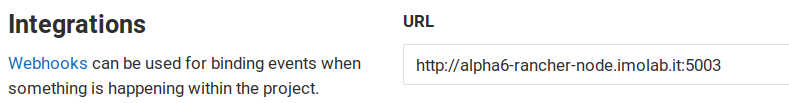
\includegraphics[width=\textwidth]{img/webhook-gitlab.png}\\
    \caption[Webhook, GitLab]{Inserimento URL per configurare un webhook su un progetto (GitLab)}
\end{figure}


\subsubsection{Eventi supportati}
Segue la lista degli eventi supportati dal Producer GitLab:
\begin{itemize}
    \item Push events
    \item Comments
    \item Issues events
\end{itemize}

% TODO: Resto delle attività utile all'amministratore che configura l'applicazione


\subsection{Gestore Personale}

Il Gestore Personale è la componente principale di Butterfly. %che tiene la logica di business di Butterfly.
Esso si può distinguere in due sotto-componenti:

\begin{itemize}
    \item Interfaccia utente
    \item Message processor, che tiene la logica di business di Butterfly
\end{itemize}

Il Message processor non è di pertinenza di questo manuale, per cui verrà discusso l'utilizzo del sistema tramite
l'interfaccia utente.

% \subsection{Interfaccia utente}

\subsubsection{Iscrizione a Butterfly}

Per iscriversi a Butterfly, accedere all'interfaccia web tramite il link

\begin{center}
    \url{link/pannello/utente}
\end{center}

Tramite il form apposito, selezionare il bottone ``Iscrizione'' e inserire delle credenziali valide.

È necessario inserire almeno un campo tra e-mail e Telegram, per avere un'identificativo univoco
all'interno del sistema.

È anche possibile inserire un nuovo utente tramite API Rest. Vedere la sezione apposita.


\subsubsection{Modifica preferenze}

\subsubsection{Inserimento giorni di indisponibilità}

\subsubsection{Aggiunta progetti e priorità}

\subsubsection{Disiscrizione}


\subsection{API Rest}

Per Butterfly abbiamo utilizzato lo standard API Rest per la gestione delle risorse.
Viene descritto nelle prossime sezioni come interagire con le API del sistema.

\subsubsection{Users}

\texttt{Users} è la risorsa che corrisponde agli utenti.
È possibile visualizzare, aggiungere, modificare o rimuovere gli utenti tramite una semplice
richiesta HTTP.

\paragraph{Visualizzazione}

\begin{itemize}
    \item \textbf{Payload di tutti gli utenti}: \texttt{GET /users}
    \item \textbf{Utente specifico}: \texttt{GET /users/<id>}
\end{itemize}

\paragraph{Inserimento}
    è possibile inserire un nuovo utente tramite la richiesta
    \begin{center}
        \texttt{POST /users}
    \end{center}

È
\begin{table}[H]
    \begin{paddedtablex}[1.7]{\textwidth}{cXc}%0 opz  2 obb

        \bottomrule
    \end{paddedtablex}
    \caption{Elenco dei requisiti di funzionalità (\thetableCounter)}
\end{table}

\subsection{Configurazione piattaforma di messaggistica}

\subsubsection{Email}

Per ricevere i messaggi di Butterfly tramite e-mail, è sufficiente fornire tramite l'interfaccia del Gestore Personale l'e-mail sulla
quale si vuole ricevere la notifica.

\subsubsection{Telegram}

Per ricevere le notifiche via Telegram, è necessario fare un passaggio addizionale. Va fornita l'autorizzazione al bot per poter inviare messaggi
agli utenti. Il bot è raggiungibile al seguente link:
\begin{center}
    \url{http://t.me/ButterflyBot}
\end{center}

Dare il comando \texttt{/start} per dare l'autorizzazione di inoltro dei messaggi al bot.
È necessario inoltre aggiungere tramite l'interfaccia del Gestore Personale il proprio account Telegram.
